\documentclass[12pt, letterpaper]{article}
\usepackage[french]{babel}
\usepackage{graphicx}
\usepackage{blindtext}
\usepackage{multicol}
\graphicspath{{images/}}
\usepackage{hyperref}
\usepackage[T1]{fontenc} 
\usepackage{fancyhdr}
\usepackage{wrapfig}

\title{Rapport de stage de seconde}
\author{Tristan KERMORVANT}
\date{16-27 juin 2025}

\makeatletter

\begin{document}
\pagestyle{fancy}
\fancyhead{} 
\fancyhead[L]{\textsc{\@author}}
\fancyhead[C]{16-27 juin 2025}
\fancyhead[R]{2nde 3}

\thispagestyle{empty}

\vspace*{-3cm}
\noindent \makebox[\textwidth]{%
    \@date \hfill 2\scriptsize nde \normalsize 3
}

\vspace{4cm}

\begin{center}
    \LARGE \sc \@title
    \vskip 0.5in
    
    \includegraphics[height=35mm]{INRIA}
    
    \vskip 0.45in
    {\large \@author}
    \vfill
\end{center}

\vspace{3cm}

\begin{center}
    \normalfont
    Responsable de stage : Marie GENERALI
\end{center}

\newpage

\tableofcontents

\section{Présentation de l'entreprise}

\subsection{Fiche synthétique}
\begin{center}

\begin{minipage}[t]{0.55\textwidth}
    \begin{description}
        \item[Date de fondation :] 1967
        \item[Type :] Établissement public à caractère scientifique et technologique
        \item[Effectif total :] 4 800+ dont scientifiques chercheurs \tiny(2024)\normalsize
        \item[Président :] \href{https://fr.wikipedia.org/wiki/Bruno_Sportisse}{Bruno Sportisse}
        \item[Budget :] 307 millions \tiny(2024)\normalsize
        \item[Affiliation :] Ministère de l'Éducation nationale, de l'Enseignement supérieur et de la Recherche
    \end{description}
\end{minipage}
\hfill
\begin{minipage}[t]{0.4\textwidth}
    \textbf{Centres de l'Inria:}\\[0.5em]
    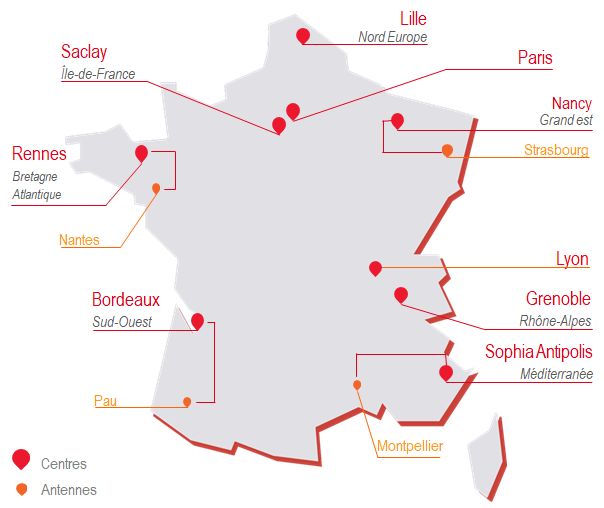
\includegraphics[width=\textwidth]{centres}
\end{minipage}

\end{center}



\subsection{Qu'est-ce que l'INRIA ?}
Fondé en 1967, Inria, ou Institut national de recherche en informatique et en automatique, est un établissement public à caractère scientifique et technologique.
Initialement créé sous le nom d'IRIA, il est conçu pour piloter l'axe recherche du \og plan Calcul\fg, une initiative stratégique visant à renforcer l'indépendance technologique de la France en informatique face à la domination américaine dans ce domaine.

Dans les années 1970, il développe notamment le projet \emph{Cyclades}, un réseau de communication pionnier, rivalisant avec Arpanet aux États-Unis, qui a inspiré la création d'Internet.
En 1980, l'IRIA devient l'I\emph{N}RIA, qui traduit l'ancrage désormais national de L'Institut.

L'objectif initial de l'INRIA et de \og Pourvoir la France en technologies de pointe et développer son autonomie et sa souveraineté\fg.

\vspace{5mm}

Aujourd'hui, l'institut se présente comme l'\emph{institut national de recherche dans les sciences et technologies du numérique}. Ses missions sont dans les domaines de l'informatique, de l'automatique et des
mathématiques appliquées de promouvoir la recherche, l'innovation et la formation.

\begin{quotation}
    \og Porter la révolution du numérique par les mathématiques et l'informatique.\fg \cite{mission-inria}
\end{quotation}

L'Inria possède de nombreux centres de recherche répartis sur le territoire français. Son siège est situé à Rocquencourt, à proximité de Versailles, et j'ai effectué mon stage au centre de Saclay, au coeur de la technopole Paris-Saclay.
\begin{figure}[h]
    \centering
    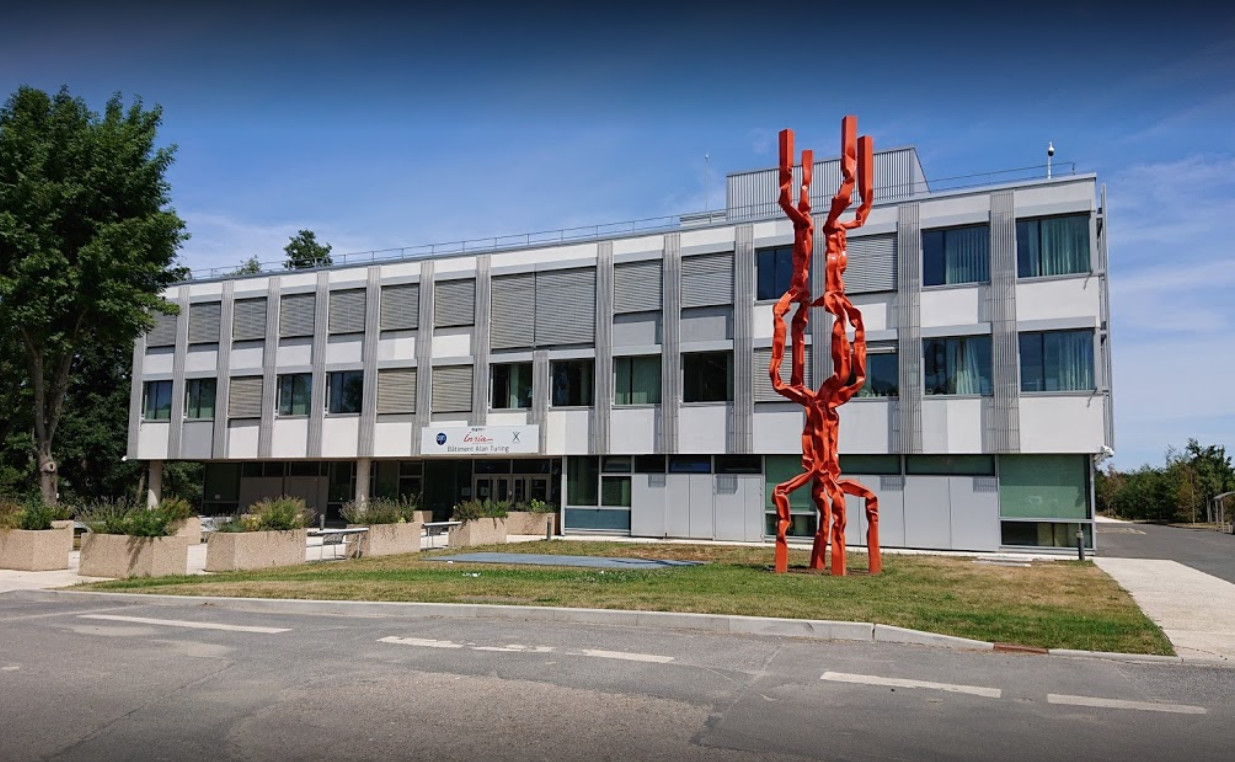
\includegraphics[height=0.28\textwidth]{inria_saclay}
    \hspace{1em}
    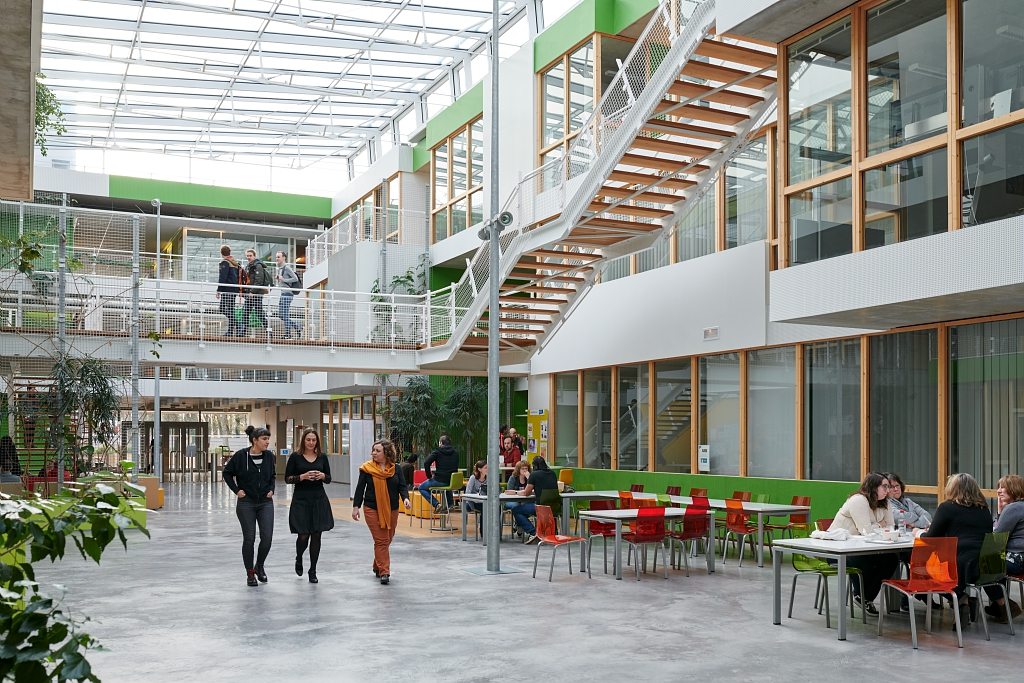
\includegraphics[height=0.28\textwidth]{interieur}
    \caption{Le bâtiment Turing à Palaiseau, sur le campus de l'École polytechnique et son intérieur.}
\end{figure}

Les centres sont eux-mêmes divisés en équipes de recherche, dont celle dans laquelle j'ai effectué mon stage, SODA.

\subsection{Présentation de l'équipe SODA}

L'équipe SODA mène des recherches à l'intersection de l'apprentissage automatique, des bases de données et des sciences sociales quantitatives.

\begin{quotation}
    \og Nous contribuons des outils d'apprentissage statistique pour répondre à des questions de science des données, typiquement sur des données relationnelles. Nos applications principales sont la santé et l'éducation.\fg \cite{soda}
\end{quotation}

\begin{figure}[h]
    \centering
    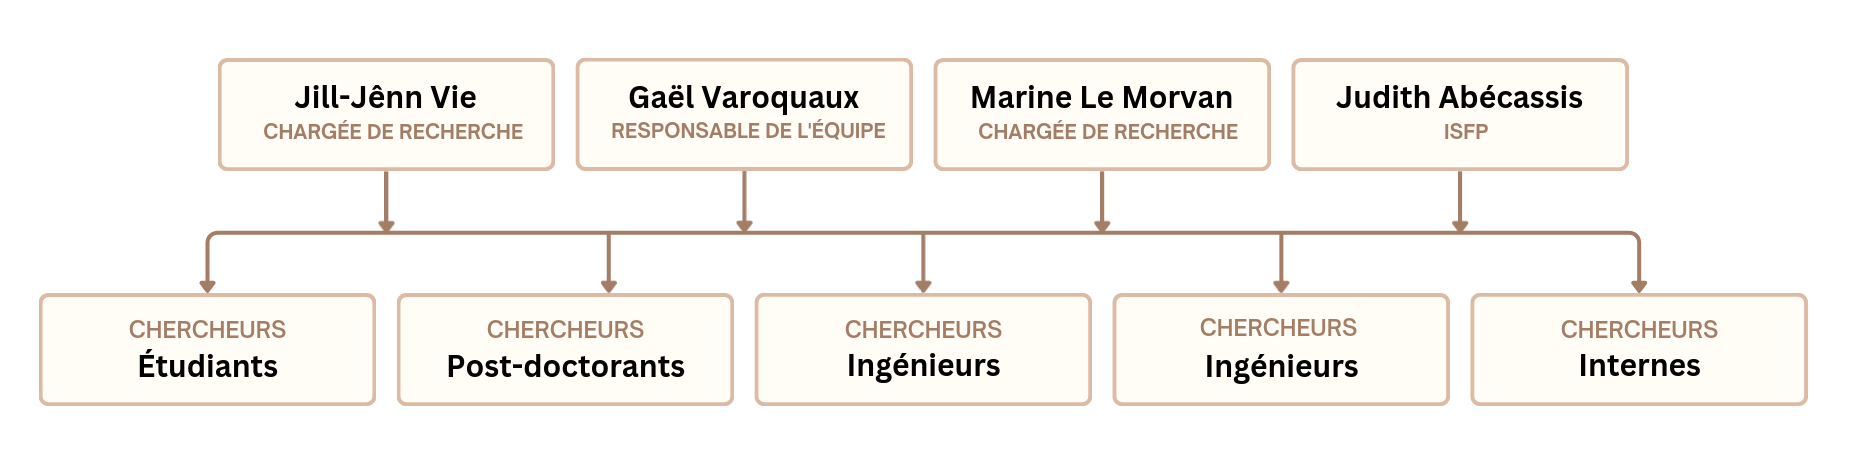
\includegraphics[width=1\textwidth]{organigramme}
    \caption{Organisation de l'équipe SODA.}
\end{figure}

Ils maintiennent notamment le logiciel \href{https://https://scikit-learn.org/}{Scikit-learn}, la bibliothèque la plus utilisée pour l'apprentissage automatique en Python. 

\begin{figure}[h]
    \centering
    
\includegraphics[height=0.1\textwidth]{soda}
    \hspace{1em}
    
\includegraphics[height=0.1\textwidth]{scikit-learn}
    \caption{Logo de l'équipe SODA et du logiciel Scikit-learn.}
\end{figure}


\pagebreak
\section{Mon travail de stage}
\subsection{Intelligence artificielle et apprentissage automatique}

L'intelligence artificielle est une discipline scientifique qui vise à faire réaliser par des machines des tâches mettant en \oe{}uvre des fonctions cognitives 
humaines : perception, language, raisonnement, plannification, mouvement. Elle est à la frontière entre l'informatique, 
la statistique, les mathématiques, les sciences cognitives et la philosophie.

L'apprentissage automatique ou machine learning est un domaine de l'intelligence artificielle. C'est une technique
permettant aux algorithmes d'intelligence artificielle de s'entraîner et d'apprendre grâce à
des exemples, sans avoir été préalablement programmés spécifiquement à cet effet.
L'entraînement de tels algorithmes nécessite une grande quantité de données
sur lesquelles entraîner les modèles.

Il existe plusieurs types d'apprentissage automatique, dont l'un des plus commun, l'apprentissage supervisé, qui consiste à entraîner un modèle sur un
 ensemble de données étiquetées et de le tester sur un ensemble de données disjoint afin d'évaluer ses performances ou mesurer les biais qu'il peut contenir. 

\subsection{Problématiques des biais et de l'équité}

    \subsubsection*{D'où viennent les biais dans les modèles d'IA ?}
    Les systèmes d'IA basés sur l'apprentissage automatique apprennent à partir de jeux de données existants, reflétant des pratiques humaines. Lorsque ces données 
    contiennent des biais sociétaux (inégalités, discriminations ou stéréotypes), les algorithmes peuvent involontairement les reproduire, car ils sont programmés 
    à imiter ce qu'ils voient. Bien que le traitement des données soit mathématiquement neutre, les préjugés présents dans les données d'entraînement se retrouvent 
    ainsi répliqués dans les résultats du modèle.

    \subsubsection*{Comment se manifestent-ils ?} 
    Les biais algorithmiques se concrétisent par des prédictions discriminantes ou des représentations stéréotypées.
    Dans un algorithmes d'évaluation de candidatures, par exemple, un biais pourrait se traduire par une discrimination à l'embauche envers certains groupes sociaux ou ethniques.

    Un algorithme de recommandation de contenu pourrait renforcer des stéréotypes en suggérant des contenus basés sur des préférences biaisées.
    
    Ou encore, une IA de génération d'images pourrait produire des représentations stéréotypées de certaines professions, en associant par exemple les femmes à des rôles de secrétaires ou d'infirmières, tandis que les hommes seraient associés à des rôles de PDG ou de scientifiques.


    \begin{figure}[h]
        \centering
        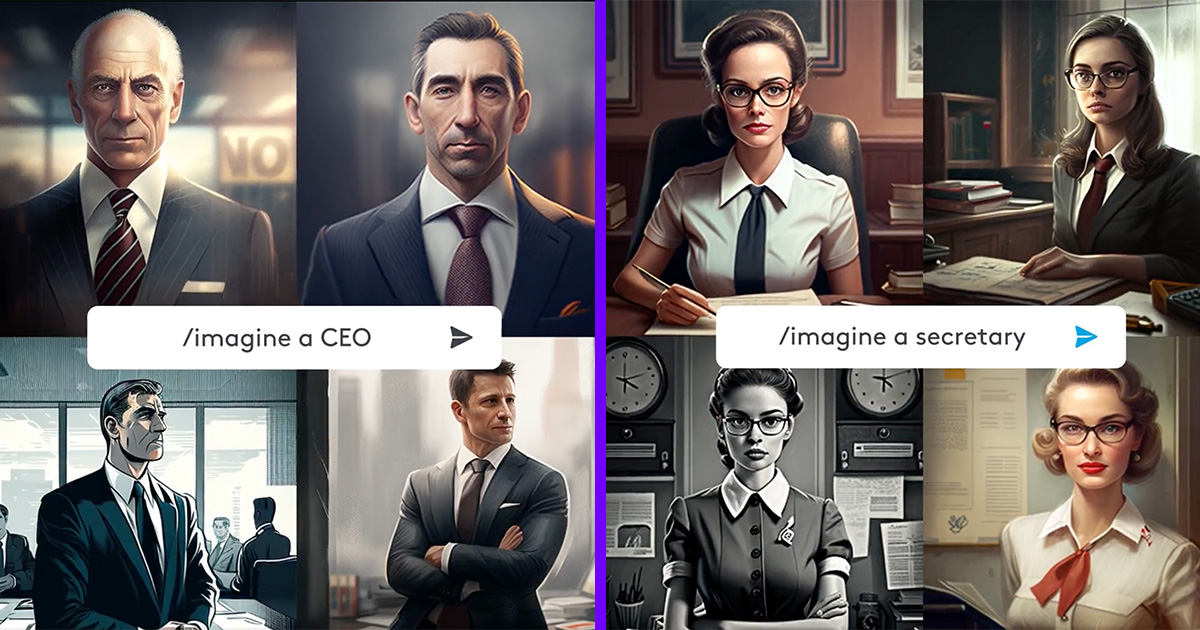
\includegraphics[width=0.8\textwidth]{midjourney-biaised}
        \caption{L'AI générative \emph{Midjourney} générant des images de PDG et de secrétaires. © Havas Paris / Presse}
    \end{figure}


    \subsubsection*{Pourquoi sont-ils problématiques ?}
    Les biais algorithmiques sont problématiques car ils renforcent les inégalités sociales et perpétuent les stéréotypes. Ils peuvent conduire à des décisions injustes, 

    Aux États-Unis, la police utilise un algorithme de prédiction de récidive criminelle. Cette IA cible deux fois plus les accusés noirs que les accusés blancs. \cite{penal}

    Dans la plupart des algorithmes, les prédictions ne sont pas accompagnées d'explications, ne permettant pas de comprendre leur fonctionnement qui est souvent perçu comme une boîte noire.
    Les biais sont donc implicites et difficiles à identifier, ce qui rend notre emprise sur eux très limitée.

\subsection{Méthodes d'atténuation des biais}

\subsubsection*{Qu'est ce que la fairness ?}
L'équité (fairness) en machine learning consiste à éviter que les modèles apprennent ou reproduisent des biais envers certains groupes 
(par exemple selon le sexe, la race, l'âge, etc.). Il existe trois grandes approches pour rendre un modèle plus juste.

\begin{enumerate}
    \item Pré-traitement (\emph{pre-processing}) :
    On agit avant l'apprentissage, en modifiant les données d'entraînement.
    \begin{itemize}
        \item Supprimer les variables sensibles (sexe, ethnie, etc.)
        \item Rééquilibrer la base de données entre les groupes
        \item Modifier ou corriger les étiquettes (labels)
    \end{itemize}
    \textbf{Avantages :} simple, compatible avec tous les modèles \\
    \textbf{Limites :} ne garantit pas l'équité finale parfaite

    \item Entraînement équitable (\emph{in-processing}) : On agit pendant l'apprentissage, en modifiant le fonctionnement du moldèle.
    \begin{itemize}
        \item Ajouter une pénalité de biais dans la fonction d'entraînement
        \item Contraindre le modèle à respecter certaines propriétés d'équité
    \end{itemize}
    \textbf{Avantages :} flexible et puissant \\
    \textbf{Limites :} nécessite des algorithmes spécifiques, peut être complexe à implémenter

    \item Ajustement des décisions (\emph{post-processing}) : On agit après l'apprentissage, en corrigeant les prédictions du modèle.
    \begin{itemize}
        \item Ajuster le seuil de décision pour chaque groupe
        \item Recalibrer les probabilités de sortie
        \item Forcer une égalité de taux entre les groupes
    \end{itemize}
    \textbf{Avantages :} simple à mettre en place, sans réentraîner le modèle \\
    \textbf{Limites :} peut être arbitraire ou perçu comme injuste

\end{enumerate}

Ma tâche durant ce stage a été d'expérimenter avec les differentes méthodes d'atténuation des biais en comparant également les performances et l'équité de différents modèles d'intelligence artificielle.

\subsection{Experimentation}

\subsubsection{Données}
Le jeu de donnée est celui d'étudiants en droit, contenant de nombreuses informations comme l'éthnie, le sexe, le score au test d'entrée en école de drotit, la moyenne des études universitaires, etc. sur plus de 20 000 étudiants.
Il est utilisé pour prédire si un étudiant réussira ou non son examen de fin de première année. Un extrait du jeu de données est présenté sur la figure \ref{fig:law_data}.

\begin{figure}[h!]
    \centering
    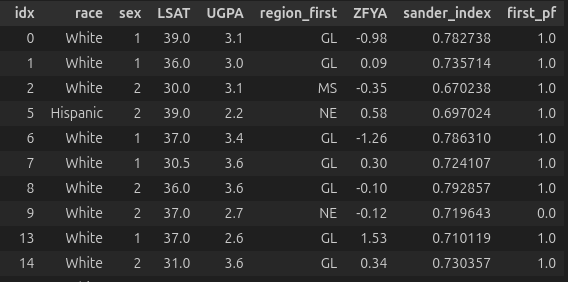
\includegraphics[width=0.8\textwidth]{law_data}
    \caption{Extrait du jeu de données d'étudiants en droit.}
    \label{fig:law_data}
\end{figure}

La première étape consiste à visualiser le jeu de données pour tenter d'identifier des biais qu'il pourrait contenir.
Dès lors, on remarque sur la figure \ref{fig:success_rate} que les étudiants blancs ont une moyenne de réussite grandement supérieure à celle des étudiants noirs ou amérindiens, de même pour les notes.

\begin{figure}[h!]
    \centering
    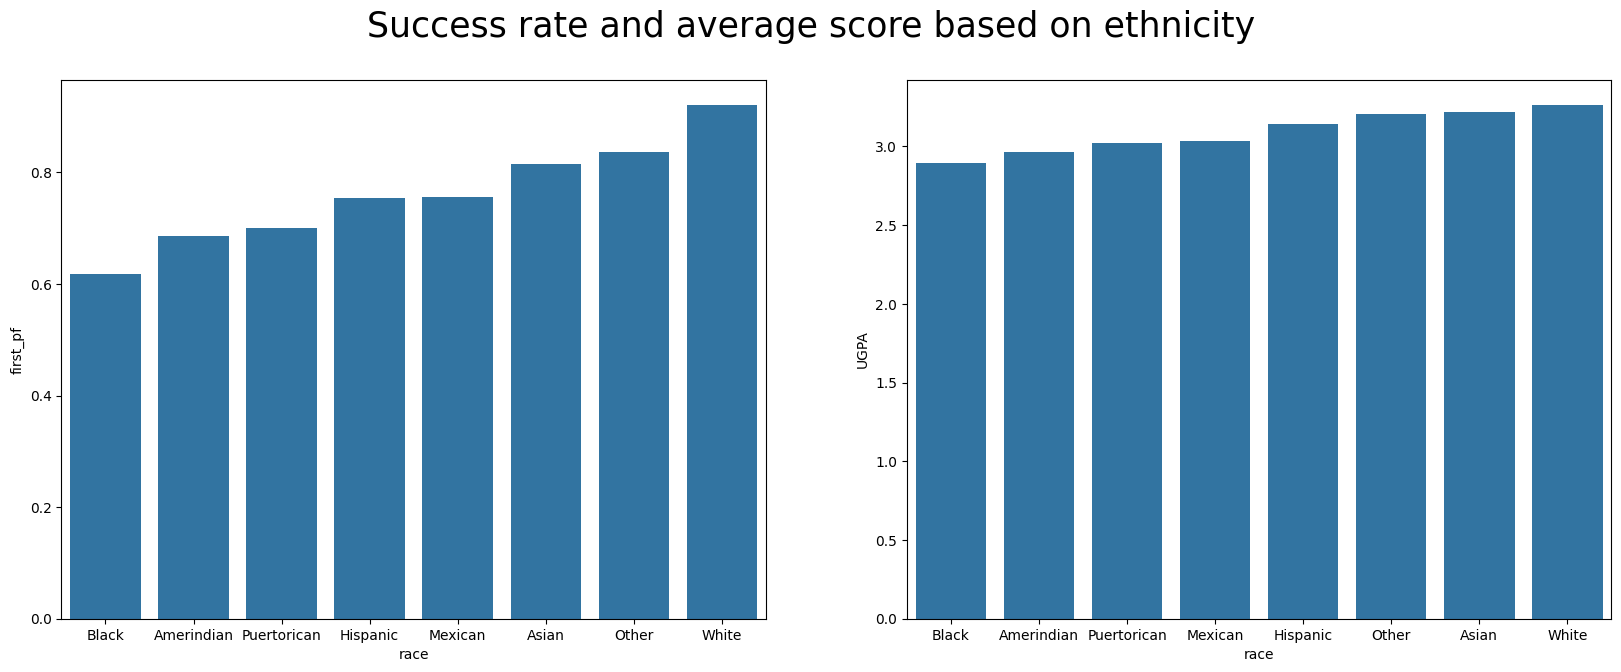
\includegraphics[width=0.8\textwidth]{success_rate}
    \caption{La moyenne de réussite des étudiant et leur des notes en fonction de leur ethnie.}
    \label{fig:success_rate}
\end{figure}

De plus, on remarque que les étuidiants blancs sont sur-représentés dans le jeu de données, constituant la quasi totalité des étudiants, à hauteur de 83,9\%. Figure \ref{fig:count}. Cela constitue donc un biais que l'on pourra exploiter.

\begin{figure}
    \centering
    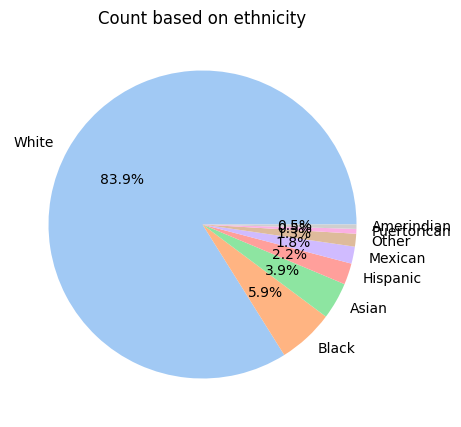
\includegraphics[width=0.6\textwidth]{count_race}
    \caption{Répartition des étudiants en fonction de leur ethnie.}
    \label{fig:count}
\end{figure}

Néanmoins, on ne remarque pas de réelle différence entre les étudiants masculins et féminins, ni dans la moyenne de réussite, ni dans les notes. On peut donc supposer que le sexe n'est pas un facteur de biais dans ce jeu de données. Figure \ref{fig:success_sex}

\begin{figure}
    \centering
    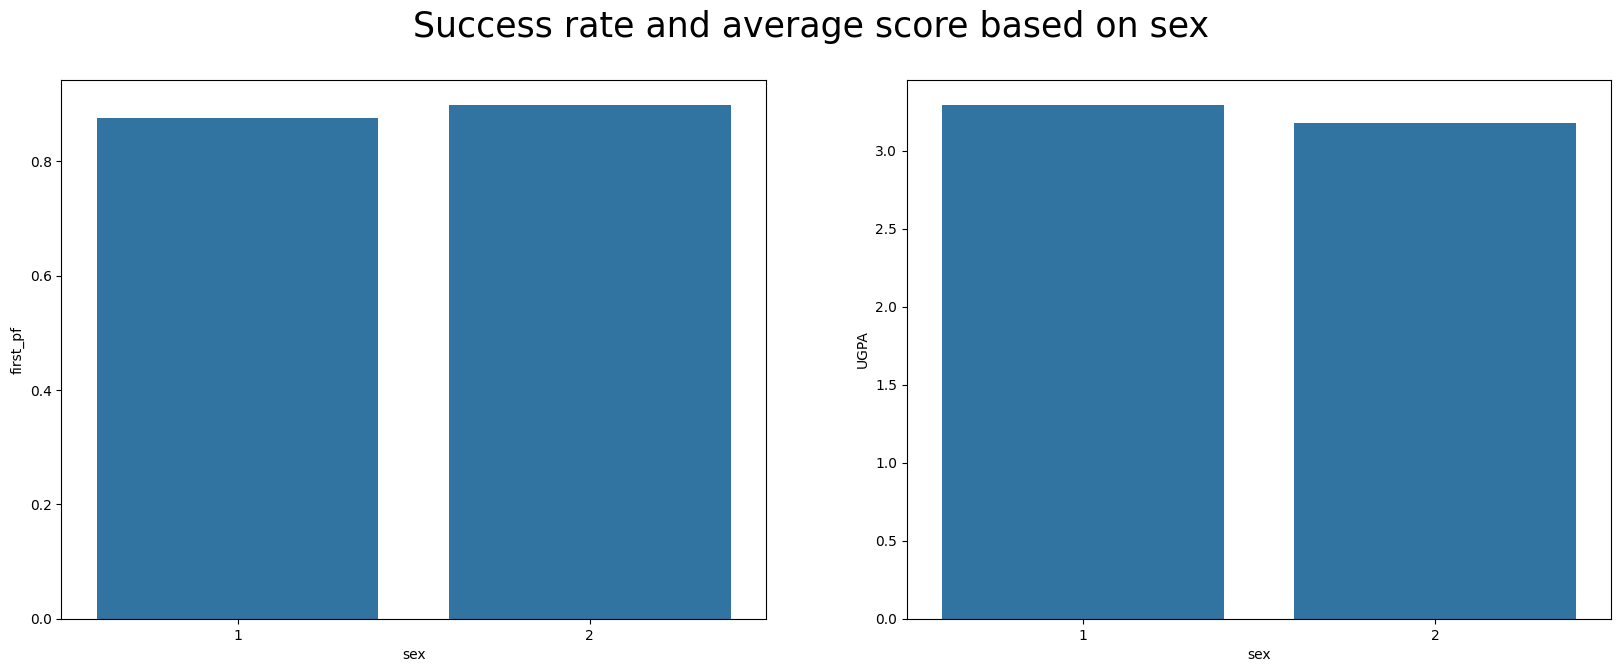
\includegraphics[width=0.6\textwidth]{success_sex}
    \caption{Répartition des étudiants en fonction de leur sexe.}
    \label{fig:success_sex}
\end{figure}

Par la suite, on utilisera donc le biais lié à l'éthnie que l'on tentera de réduire grâce aux différentes méthodes d'atténuation des biais.

\subsubsection{Modèles}

J'ai testé les performances de trois algorithmes d'intelligence artificielle différents, mais par simplicité, je n'en presenterai ici que deux.

\subsubsection*{La régression logistique}
La régression logistique est un algorithme statistique simple qui utilise une fonction affine ansi qu'une fonction sigmoïde pour prédire la probabilité d'appartenance à une classe. Il est souvent utilisé pour des problèmes de classification binaire.

\begin{figure}[h]
    \centering
    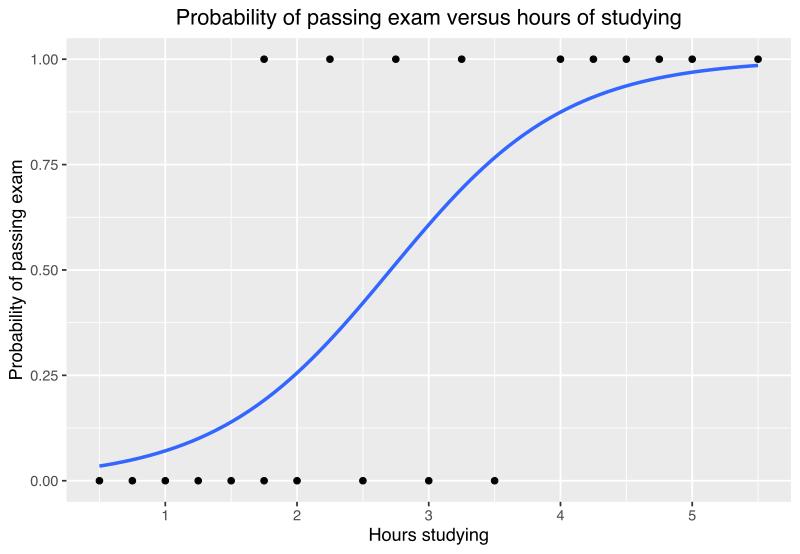
\includegraphics[width=0.6\textwidth]{logistic}
    \caption{Courbe d'une régression logistique à une dimension. © Wikipedia}
\end{figure}

\subsubsection*{Les réseaux de neurones}
Les réseaux de neurones sont des modèles informatiques inspirés du fonctionnement du
cerveau humain. Ils sont constitués de couches de neurones interconnectés, où chaque
neurone est une unité de traitement simple. Ils possèdent trois types de couches : la couche
d'entrée, les couches cachées et la couche de sortie.
La couche d'entrée comporte toutes les informations que l'on donne au modèle, cela peut être les données 
d'une image ou ici les informations sur les étudiants par exemple. Les neurones des couches cachées vont alors effectuer des 
opérations sur les valeurs de la couche d'entrée, qui vont permettre de prendre une décision en sortie. À chaque itération 
d'entrainement, l'algorithme d'apprentissage va modifier les 
paramètres de chaque neurone (qu'on appelle poids) pour se rapprocher de la sortie voulue. 

Plus il y a de couches cachées et de neurones, plus le modèle est complexe et long à
entraîner, mais plus il peut réaliser des tâches complexes. Ici, j'utilise un réseau à une seule couche, dit linéraire.

\begin{figure}[h]
    \centering
    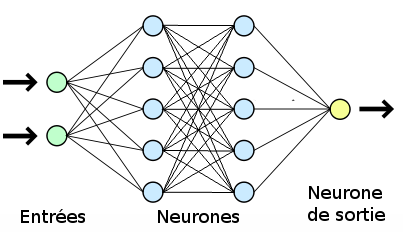
\includegraphics[width=0.6\textwidth]{neural}
    \caption{Schéma d'un réseau de neurones.}
\end{figure}

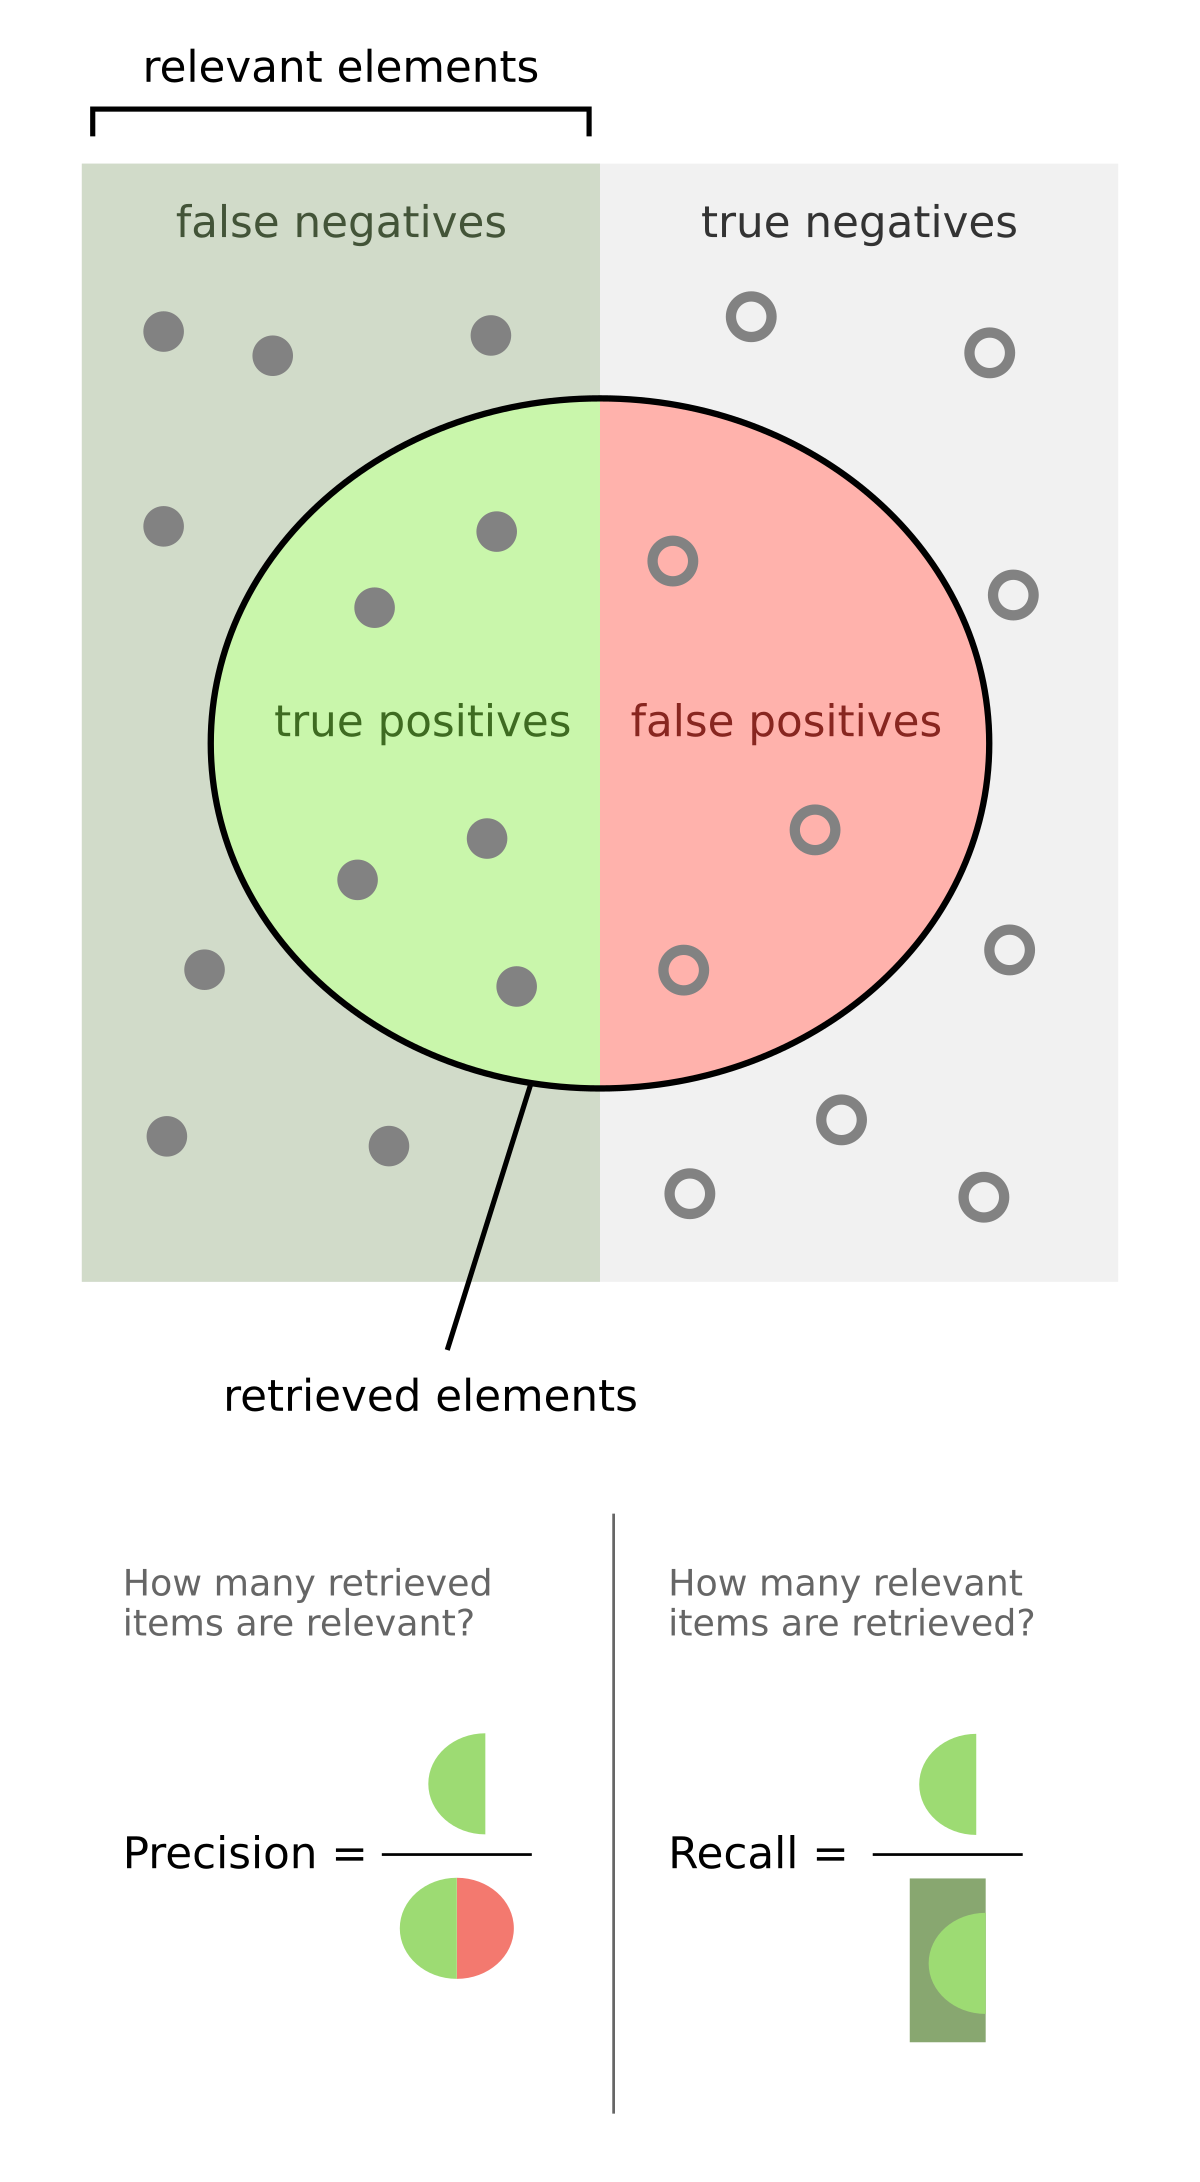
\includegraphics[width=0.4\textwidth]{precision_recall.png}

Voici la performance du réseau de neurones. La précision et le rappel sont deux métriques de performance utilisées pour 
évaluer les modèles d'apprentissage automatique. La précision mesure la proportion de prédictions correctes parmi 
toutes les prédictions faites, tandis que le rappel mesure la proportion de positives parmis celles qui auraient 
dû être prédites. 

Sur le \emph{classification report} Table \ref{tab:classification_report}, on remarque une faible performance du modèle sur la prédiction \emph{0}, qui correspond à 
l'échec de l'examen de fin de première année, mais on constate que la classe \emph{1} est bien plus représentée 
que la classe \emph{0} (5853 contre 685), ce qui explique la grande performace du modèle sur cette classe.

\begin{table}[h!]
    \centering
    \begin{tabular}{lcccc}
    \hline
    \textbf{Class} & \textbf{Precision} & \textbf{Recall} & \textbf{F1-score} & \textbf{Support} \\
    \hline
    0.0 & 0.57 & 0.31 & 0.40 & 685 \\
    1.0 & 0.92 & 0.97 & 0.95 & 5853 \\
    \hline
    \textbf{Accuracy} & & & 0.90 & 6538 \\
    \textbf{Macro avg} & 0.75 & 0.64 & 0.67 & 6538 \\
    \textbf{Weighted avg} & 0.89 & 0.90 & 0.89 & 6538 \\
    \hline
    \end{tabular}
    \caption{Classification report pour le réseau de neurones.}
    \label{tab:classification_report}
\end{table}

\subsubsection{Méthode de réduction des biais}

\subsubsection*{Pré-traitement : \emph{Correlation Remover}}
La méthode de pré-traitement \emph{Correlation Remover} consiste à supprimer la corrélation entre les 
variables sensibles (ici l'ethnie) et les autres variables du jeu de données. Elle a été réalisée sur le modèle de régression logisitique.

Pour quantifier l'équité, on utilise la métrique \emph{demographic parity}, qui assure que la proportion d'appartenace à chaque groupe est indépendante de la variable sensible.
Il existe deux mesures, comprises entre 0 et 1, qui quantifient cette métrique : la \emph{demographic parity difference} et la \emph{demographic parity ratio}.
La première doit tendre vers 0 et la seconde vers 1 pour que l'équité soit respectée.
Plus d'informations sur \url{https://fairlearn.org/main/user_guide/assessment/common_fairness_metrics.html}

On observe sur le tableau \ref{tab:correlation_remover_parity} que l'équité est entièrement respectée, neanmoins, on remarque que sur la figure \ref{fig:correlation} que la performance du modèle est devenue nulle, car en supprimant 
la corrélation entre les variables sensibles et les autres variables, on supprime également une information sans doute nécessaire à la prédiction de la variable cible.

\begin{table}[h!]
    \centering
    \begin{tabular}{lcc}
        \hline
        & \textbf{Avant} & \textbf{Après} \\
        \hline
        Demographic parity difference & 0.35 & 0.00 \\
        Demographic parity ratio      & 0.65 & 1.00 \\
        \hline
    \end{tabular}
    \caption{Évolution des métriques d'équité (\emph{demographic parity}) avant et après la méthode \emph{Correlation Remover}.}
    \label{tab:correlation_remover_parity}
\end{table}

\begin{figure}[h]
    \centering
    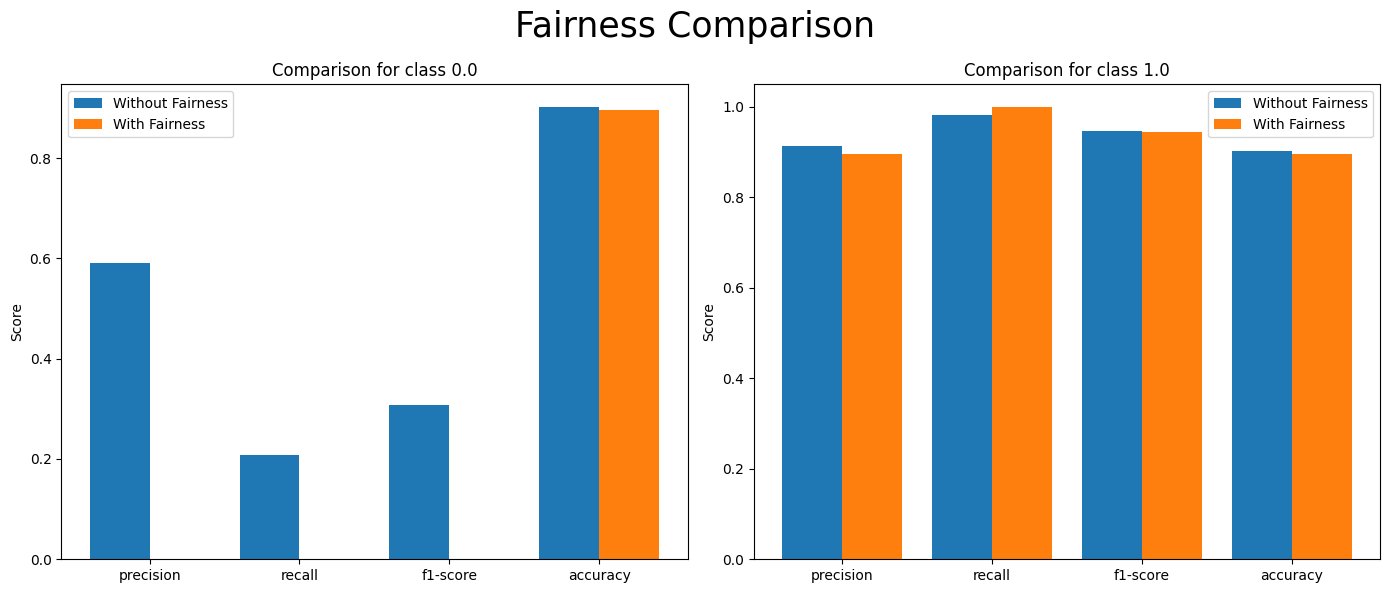
\includegraphics[width=0.6\textwidth]{cr}
    \caption{Résultat de la méthode \emph{Correlation Remover} sur le jeu de données.}
    \label{fig:correlation}
\end{figure}

\subsubsection*{In-processing : \emph{pénalité d'équité}}
Cette méthode a été implémentée sur le réseau de neurones car il est très facile d'ajouter une pénalité dans 
la fonction de perte, c'est à dire durant la boucle d'entraînement de l'algorithme.
Elle consiste à calculer la métrique d'équité \emph{demographic parity} à chaque itération d'entraînement et à ajouter une pénalité dans la fonction de perte si cette métrique n'est pas respectée.
À force, le modèle apprend à respecter l'équité tout en essayant de maximiser la performance.

\begin{table}[h!]
    \centering
    \begin{tabular}{lcc}
        \hline
        & \textbf{Avant} & \textbf{Après} \\
        \hline
        Demographic parity difference & 0.45 & 0.37 \\
        Demographic parity ratio      & 0.54 & 0.62 \\
        \hline
    \end{tabular}
    \caption{Évolution des métriques d'équité (\emph{demographic parity}) avant et après la pénalité d'équité (in-processing) sur le réseau de neurones.}
\end{table}

On remarque une amélioration de l'équité, plus légère, néanmoins la performance du modèle est restée quasi semblable, comme on peut le voir sur la figure \ref{fig:inprocessing}.

\begin{figure}[h]
    \centering
    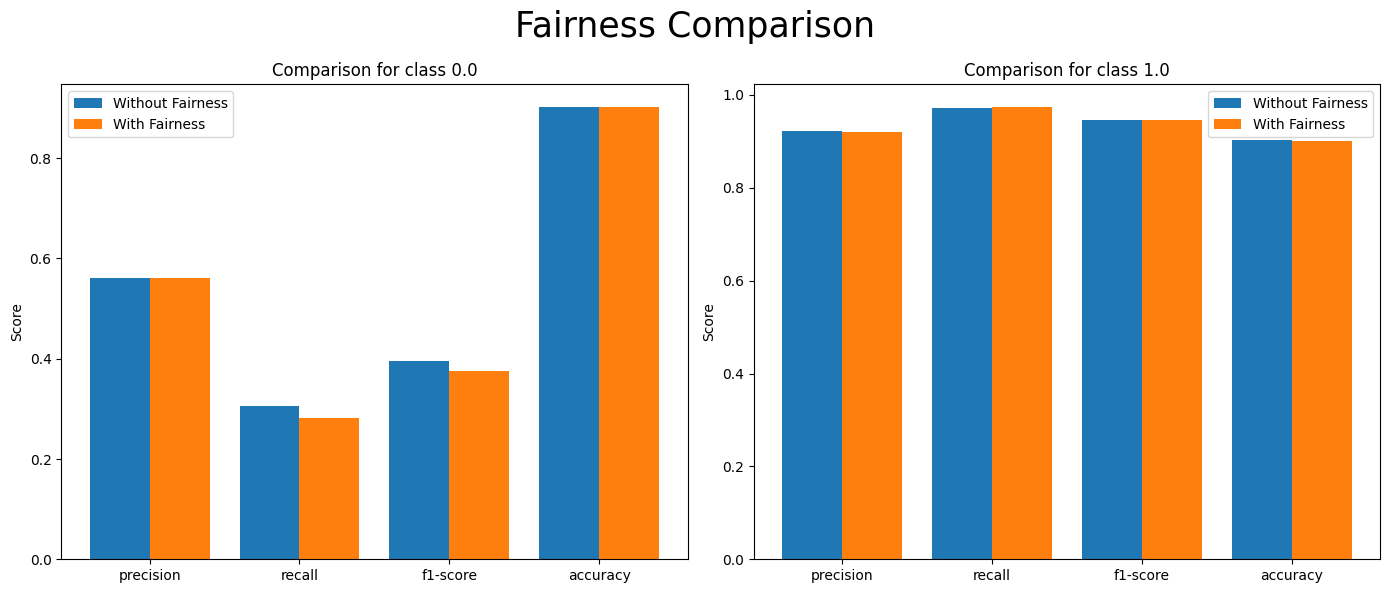
\includegraphics[width=0.6\textwidth]{inprocessing}
    \caption{Résultat de la pénalité d'équité sur le réseau de neurones.}
    \label{fig:inprocessing}
\end{figure}

\subsubsection*{{Post-processing : \emph{Threshold Optimization}}}
Cette méthode consiste à ajuster le seuil de décision du modèle pour chaque groupe afin de respecter l'équité.
C'est l'équivalent à faire des "quotas" pour chaque groupe, en ajustant le seuil de décision pour que la proportion de prédictions positives soit égale entre les groupes.
Elle a été effectuée sur le modèle de régression logistique.

\begin{figure}
    \centering
    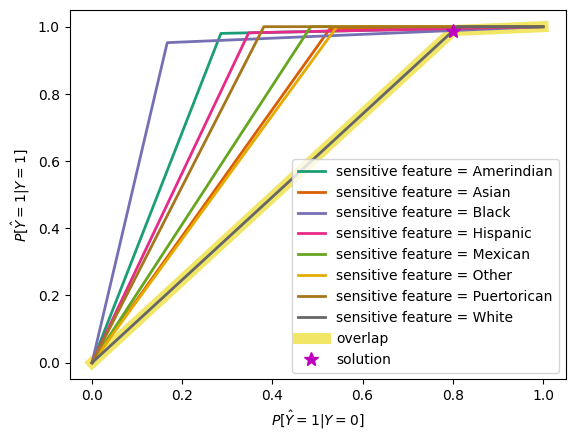
\includegraphics[width=0.6\textwidth]{threshold_opti}
    \caption{Les seuils de décision pour chaque groupe, où la classe Black est "avantagée"}
    \label{fig:threshold_opti}
\end{figure}

\begin{table}[h!]
    \centering
    \begin{tabular}{lcc}
        \hline
        & \textbf{Avant} & \textbf{Après} \\
        \hline
        Demographic parity difference & 0.35 & 0.07 \\
        Demographic parity ratio      & 0.65 & 0.93 \\
        \hline
    \end{tabular}
    \caption{Évolution des métriques d'équité (\emph{demographic parity}) avant et après la méthode de \emph{Threshold Optimization}.}
\end{table}

On remarque une amélioration significative de l'équité, mais la performance du modèle a donc été également dégradée, cependant 
moins que la méthode de pré-traitement comme on peut le voir sur la figure \ref{fig:threshold_opti_results}.

\begin{figure}
    \centering
    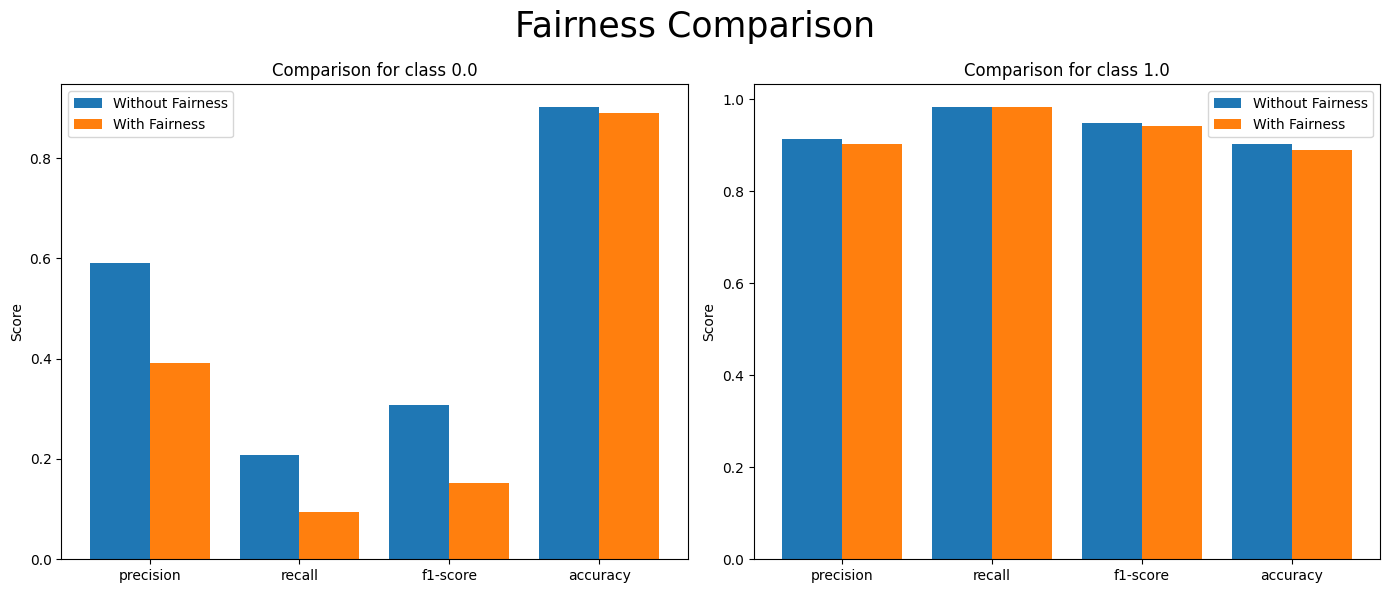
\includegraphics[width=0.6\textwidth]{threshold_opti_results}
    \caption{Résultat de la méthode de \emph{Threshold Optimization}.}
    \label{fig:threshold_opti_results}
\end{figure}

\subsubsection{Analyse et interprétation}
La méthode de pré-traitement \emph{Correlation Remover} et de post-processing \emph{Threshold Optimization} ont permis d'atteindre une équité parfaite, cependant les modèles ont perdu toute capacité de prédiction.
La méthode d'in-processing, la pénalité d'équité, a permis d'améliorer l'équité du modèle de manière significative, mais sans dégrader la performance du modèle, ce qui est un bon compromis.

On a pu observer que grâce à ces différentes méthodes, on a pu améliorer l'équité des modèles, mais à chaque fois au prix d'une perte de performance.
Cela soulève donc quelques questions éthiques :
\begin{itemize}
    \item Un modèle peut-il être performant et juste ?
    \item Quelles variables sont utiles ou problématiques ?
    \item Faut-il toujours un seul modèle pour tout le monde ?
\end{itemize}

\subsubsection*{Comment améliorer les résultats ?}
Pour chaque méthode, il est possible d'améliorer les résultats en ajustant l'intensité de la décorrélation ou le seuil de tolérance pour tenter de préserver la performance du modèle.
Sur la méthode d'in-processing, cela avait déjà été fait, un coefficient $\lambda$ avait été ajouté dans la fonction de perte pour ajuster l'importance de la pénalité d'équité.
Je l'avait également optimisé pour trouver le meilleur compromis entre performance et équité, mais il est possible de l'optimiser encore plus finement.

\section{Réflexions personnelles}
\subsection{Comparaison avec le stage de 3e}
Recherche privée vs recherche publique

\subsection{Activtés spécifiques au domaine de la recherche publique}
Soutenance de thèse, coding sprint, \LaTeX

\subsection{Conclusion}

\section{Remerciements}

\bibliographystyle{unsrt}
\bibliography{references}
\end{document}